% ======================================================================
%  Chapter 7 — Breaking Time Reversal
%  Dirac Berry curvature, Chern number from a pair of cones.
% ======================================================================

\section{The missing ingredient}
\label{sec:ch7-missing}

The Dirac cones derived in \chref{ch:dirac-cones} are gapless: the two
bands touch linearly at isolated points in the Brillouin zone.  The
Berry curvature is singular at the degeneracy, and the Chern number is
not defined because the bands are not separated by a gap.  To create a
topological photonic system---one with well-defined Chern numbers and
protected edge states---we must \emph{open a gap} at the Dirac points.

From the symmetry analysis of the preceding chapter, we know that Dirac
points are protected by the simultaneous presence of time-reversal
($\Top$) and inversion ($\Pop$) symmetry.  Breaking either symmetry can
lift the degeneracy.  But the topological consequences are profoundly
different.  Breaking \emph{inversion} symmetry opens a gap but
produces \emph{zero} net Chern number, because the Berry fluxes at
$K$ and $K'$ carry opposite signs and cancel exactly.  Breaking
\emph{time-reversal} symmetry, by contrast, opens a gap in which
the Berry fluxes at $K$ and $K'$ carry the \emph{same} sign and add
to give a nonzero Chern number.
In this chapter we carry out the time-reversal-breaking programme in
detail, deriving the massive Dirac dispersion, the Berry curvature of
the gapped bands, and the resulting Chern numbers.

\section{The gyrotropic perturbation}
\label{sec:ch7-gyrotropic}

\subsection{Faraday coupling in the permittivity}
\label{sec:ch7-faraday}

We return to the hexagonal photonic crystal of
\secref{sec:ch6-nfp-setup} and add a magneto-optical (Faraday)
perturbation
\cite{he2016photonic}.  An applied magnetic field along $\hat{z}$ induces
off-diagonal components in the permittivity tensor:
\begin{equation}\label{eq:ch7-faraday-eps}
  \varepsilon_{xy} = -\varepsilon_{yx}
  = \ii\,\varepsilon_0\bar\varepsilon\,\eta(\rvec,\omega)\,,
\end{equation}
where the gyrotropic function $\eta$ has the same periodicity as the
lattice:
\begin{equation}\label{eq:ch7-eta}
  \eta(\rvec,\omega) = \eta_0(\omega) + \eta_1(\omega)\,V_G(\rvec)\,.
\end{equation}
Here $\eta_0$ and $\eta_1$ are real odd functions of $\omega$ (as
required by the Hermiticity of $\Mmat$), and we assume
$|\eta_0|,|\eta_1|\ll|\lambda|\ll 1$ with negligible frequency
dependence near $\omega_D$.

The diagonal permittivity components are unchanged:
$\varepsilon_{xx}=\varepsilon_{yy}=\varepsilon_0\bar\varepsilon(1+\lambda V_G)$
as before.  The permeability remains $\mu_0\mathbf{I}$.

\begin{remark}
Alternatively, the Faraday effect can enter through the
\emph{permeability} tensor (as in magnetised ferrites), with
off-diagonal $\mu_{xy}=-\mu_{yx}=\ii\mu_0\kappa$
\cite{wang2007reflection}.  The two formulations
are related by electromagnetic duality.  We use the permittivity form
here to follow Haldane and Raghu's original treatment; the permeability
form will appear naturally in \chref{ch:microwave-crystal} when we
discuss the YIG experiment.
\end{remark}

\subsection{Effect on the material matrix}
\label{sec:ch7-material-matrix}

The Faraday perturbation modifies the $6\times 6$ material matrix by
adding an off-diagonal anti-Hermitian block to the permittivity:
\begin{equation}\label{eq:ch7-delta-M}
  \delta\Mmat(\rvec) =
  \begin{pmatrix}
    \varepsilon_0\bar\varepsilon\,\delta\epst & \mathbf{0} \\
    \mathbf{0} & \mathbf{0}
  \end{pmatrix},
  \qquad
  \delta\varepsilon_{ij} = \ii\,\eta(\rvec)\,\epsilon_{ij3}\,,
\end{equation}
where $\epsilon_{ij3}$ is the Levi-Civita symbol.
Explicitly, $\delta\varepsilon_{12}=\ii\eta$ and
$\delta\varepsilon_{21}=-\ii\eta$, with diagonal entries zero.

Since $\delta\epst$ is Hermitian
($\delta\varepsilon_{12}^*=(-\ii\eta)^*=\ii\eta
\neq\delta\varepsilon_{12}$, but
$\delta\varepsilon_{12}^*=\delta\varepsilon_{21}^{\phantom{*}}$,
which is the Hermiticity condition), the perturbed $\Mmat$ remains
Hermitian.
However, the condition $\varepsilon_{xy}=-\varepsilon_{yx}\neq 0$
violates the reciprocity condition $\epst=\epst^T$
(\secref{sec:ch2-reciprocity}), confirming that time-reversal symmetry
is broken.

\section{Gap opening at the Dirac point}
\label{sec:ch7-gap}

\subsection{The massive Dirac equation}
\label{sec:ch7-massive-dirac}

The Faraday perturbation introduces a \emph{mass term} into the
effective $2\times 2$ Dirac equation at each Dirac point.  In
degenerate perturbation theory, the perturbation $\delta\Mmat$
projected onto the two-mode subspace at $\kvec_K$ gives a contribution
proportional to $\sigma_z$ (the Pauli matrix diagonal in the mode
basis).  The effective equation becomes
\begin{equation}\label{eq:ch7-massive-dirac}
  \boxed{%
  v_D\bigl(\delta k_x\,\sigma_x + \delta k_y\,\sigma_y\bigr)|\psi\rangle
  + v_D\kappa\,\sigma_z|\psi\rangle
  = \delta\omega\,|\psi\rangle\,,}
\end{equation}
where $\kappa$ is the \emph{Dirac mass parameter}, with dimensions of
inverse length, given by
\begin{equation}\label{eq:ch7-kappa}
  \kappa = |\kvec_K|\Bigl(
    \tfrac{3}{2}\eta_1(\omega_D) - 3\lambda\,\eta_0(\omega_D)
  \Bigr)\,
\end{equation}
The displayed formula above follows the convention and normalisation used in \cite{raghu2008analogs}.
This expression was derived by Haldane and Raghu from the matrix element
of $\delta\Mmat$ between the degenerate Dirac modes
\cite{haldane2008possible}.

\subsection{Gapped dispersion}
\label{sec:ch7-gapped-dispersion}

The eigenvalues of the massive Dirac equation \eqref{eq:ch7-massive-dirac}
are
\begin{equation}\label{eq:ch7-gapped-disp}
  \boxed{%
  \delta\omega_\pm(\delta\kvec)
  = \pm v_D\sqrt{|\delta\kvec|^2 + \kappa^2}\,.}
\end{equation}
The Dirac degeneracy is lifted: there is now a gap of width
$2v_D|\kappa|$ centred at the Dirac frequency $\omega_D$.  The
dispersion is hyperbolic, approaching the linear Dirac cone far from
the gap ($|\delta\kvec|\gg|\kappa|$) and becoming flat near
$\delta\kvec=\mathbf{0}$ ($|\delta\kvec|\ll|\kappa|$).

The sign of $\kappa$ determines which band moves up and which moves
down.  Reversing the applied magnetic field (and hence the sign of
$\eta$) reverses the sign of $\kappa$, which will be crucial for the
domain-wall construction of \chref{ch:one-way-interface}.

\section{Berry curvature of the massive Dirac model}
\label{sec:ch7-berry-curvature}

\subsection{Derivation}
\label{sec:ch7-bc-derivation}

The massive Dirac Hamiltonian $H=v_D(\delta k_x\sigma_x
+\delta k_y\sigma_y+\kappa\sigma_z)$ has the form
$H=\mathbf{d}\cdot\boldsymbol{\sigma}$ with
$\mathbf{d}=v_D(\delta k_x,\delta k_y,\kappa)$.  Using the general
result for a two-band system (Exercise~5.4):
\begin{equation}\label{eq:ch7-bc-general}
  \Omega_\pm(\delta\kvec)
  = \pm\frac{1}{2}\,\hat{\mathbf{d}}\cdot
  \Bigl(\pderiv{\hat{\mathbf{d}}}{\delta k_x}\times
        \pderiv{\hat{\mathbf{d}}}{\delta k_y}\Bigr)\,,
\end{equation}
where $\hat{\mathbf{d}}=\mathbf{d}/|\mathbf{d}|$.

Computing the derivatives and cross product:
\begin{equation}\label{eq:ch7-bc-result}
  \boxed{%
  \Omega_\pm(\delta\kvec)
  = \pm\frac{\kappa}{2\bigl(|\delta\kvec|^2+\kappa^2\bigr)^{3/2}}\,.}
\end{equation}

This is the \emph{massive Dirac Berry curvature}: a smooth, peaked
function centred at $\delta\kvec=\mathbf{0}$, with a peak value of
$\pm 1/(2\kappa^2)$ and a characteristic width $\sim|\kappa|$ in
momentum space.

\subsection{Berry flux from a single Dirac cone}
\label{sec:ch7-half-flux}

Integrating the Berry curvature over the entire $(\delta k_x,\delta k_y)$
plane:
\begin{align}\label{eq:ch7-half-chern}
  \frac{1}{2\pi}\int\Omega_\pm(\delta\kvec)\,\dd^2(\delta k)
  &= \pm\frac{1}{2\pi}\int_0^\infty
    \frac{\kappa}{2(q^2+\kappa^2)^{3/2}}\,2\pi q\,\dd q
  \notag\\
  &= \pm\frac{1}{2}\,\sgn(\kappa)\,.
\end{align}
The evaluation of the integral proceeds by substituting $q=|\kappa|\tan\theta$:
\begin{equation}
  \int_0^\infty\frac{q\,\dd q}{(q^2+\kappa^2)^{3/2}}
  = \Bigl[-\frac{1}{\sqrt{q^2+\kappa^2}}\Bigr]_0^\infty
  = \frac{1}{|\kappa|}\,.
\end{equation}
So the integral gives
$\pm\kappa/(2|\kappa|)=\pm\frac{1}{2}\sgn(\kappa)$.

Each gapped Dirac cone contributes a Berry flux of $\pm\pi$ (i.e.,
$\pm\frac{1}{2}$ in units of $2\pi$) to the band's Chern number.
A single Dirac cone gives a \emph{half-integer} contribution---this is
why isolated Dirac fermions cannot exist on a lattice (the
fermion-doubling theorem), and why the Chern number becomes integer only
when we account for both cones in the pair.

\section{Chern numbers from a pair of Dirac cones}
\label{sec:ch7-chern}

\subsection{Adding the contributions from K and K-prime}
\label{sec:ch7-KKprime}

The hexagonal Brillouin zone has two inequivalent Dirac points at $K$
and $K'$.  When time-reversal symmetry is broken by the gyrotropic
perturbation, each Dirac point opens a gap.  In the single-cone
basis used in this chapter (where
$H=v_D(\delta k_x\sigma_x+\delta k_y\sigma_y+\kappa\sigma_z)$
at \emph{both} valleys), both cones carry the same mass~$\kappa$,
because the valley chirality $\tau=\pm 1$ of \secref{sec:ch6-pairs}
has been absorbed into the choice of spinor basis at each $K$ point.

The total Chern number of the upper (+) band is therefore
\begin{equation}\label{eq:ch7-chern-total}
  \Chern_+ = \frac{1}{2}\sgn(\kappa) + \frac{1}{2}\sgn(\kappa)
  = \sgn(\kappa) = \pm 1\,.
\end{equation}
Similarly, $\Chern_-=\mp 1$.  The two bands that split from the Dirac
cones carry equal and opposite Chern numbers, and the gap between them
is topologically nontrivial.

\begin{remark}
If the gap had been opened by \emph{inversion} breaking (with TR
preserved), the Berry curvature would satisfy
$\Omega_n(\kvec)=-\Omega_n(-\kvec)$, so the contributions from $K$ and
$K'$ would cancel:
$\Chern_+=\frac{1}{2}\sgn(\kappa_K)+\frac{1}{2}\sgn(\kappa_{K'})
=\frac{1}{2}-\frac{1}{2}=0$.
This is the fundamental distinction between the two types of gap
opening, and the reason why time-reversal breaking is essential for
photonic Chern insulators \cite{nittis2020equivalence}.
\end{remark}

\subsection{The gap Chern number}
\label{sec:ch7-gap-chern}

For the bulk-edge correspondence of
\chref{ch:one-way-interface}, the relevant quantity is the \emph{gap
Chern number}: the sum of Chern numbers of all bands below the
topological gap
\cite{haldane2008reflection,chen2023berry}.  If the only nontrivial bands are the Dirac pair,
then the gap Chern number is $\Chern_{\mathrm{gap}}=\Chern_-=\mp 1$.
At a domain wall where the sign of $\kappa$ reverses, the gap Chern
number changes by $|\Delta\Chern_{\mathrm{gap}}|=2$, predicting two
unidirectional edge modes crossing the gap---one from each Dirac point.

\section{Physical requirements for the gyrotropic perturbation}
\label{sec:ch7-physical}

\subsection{Strength of the Faraday effect}
\label{sec:ch7-strength}

The gap width $2v_D|\kappa|$ must be large enough to:
\begin{enumerate}
  \item Overcome any residual inversion-symmetry breaking that might
  produce a competing trivial gap.
  \item Provide a useful bandwidth for the one-way edge modes.
  \item Keep the edge-mode localisation length
  $\ell\sim 1/|\kappa|$ significantly smaller than the physical
  size of the photonic crystal.
\end{enumerate}
In practice, this requires materials with a substantial magneto-optical
response at the operating frequency.  At microwave frequencies, ferrites
such as yttrium iron garnet (YIG) provide large gyrotropic parameters
($\kappa/|\kvec_K|\sim 10^{-2}$--$10^{-1}$); at optical frequencies,
the available Faraday rotation is much weaker, which is one of the main
challenges for realising topological photonic crystals at visible or
near-infrared wavelengths.

\subsection{Material candidates}
\label{sec:ch7-materials}

The first experimental realisations of photonic Chern insulators used
gyromagnetic ferrites:
\begin{itemize}
  \item \textbf{Yttrium iron garnet (YIG):} $\mathrm{Y_3Fe_5O_{12}}$,
  with large permeability gyrotropy at microwave frequencies
  (4--10~GHz) under moderate applied fields (0.1--0.5~T).  Used in
  the Wang et~al.\ experiment discussed in
  \chref{ch:microwave-crystal} \cite{nature2026observation}.
  \item \textbf{Bismuth iron garnet (BIG):} offers larger Faraday
  rotation at near-infrared wavelengths but with higher absorption.
  \item \textbf{Magneto-optical semiconductors:} InSb and related
  materials in strong magnetic fields can provide significant
  permittivity gyrotropy at THz frequencies.
\end{itemize}

\subsection{Quantitative gap estimates for different materials}
\label{sec:ch7-gap-estimates}

The size of the topological gap opened by the magneto-optical
perturbation depends on the gyrotropic response of the material, the
frequency regime, and the photonic crystal geometry.  The following
table summarises representative values for the three most commonly used
platforms \cite{ozawa2018topological,haldane2008possible}.

\begin{center}
\begin{tabular}{lccc}
  \toprule
  \textbf{Material} & \textbf{Frequency} & $\kappa_\mu/\mu_\perp$
    & \textbf{Relative gap} \\
  \midrule
  YIG (ferrite) & $4$--$5\;\mathrm{GHz}$ & $0.3$--$0.5$ &
    $3$--$5\%$ \\
  Bi:YIG (bismuth ferrite) & $1$--$3\;\mathrm{GHz}$ & $0.1$--$0.3$ &
    $1$--$3\%$ \\
  InSb (magneto-plasma) & $0.3$--$1\;\mathrm{THz}$ & $0.05$--$0.2$ &
    $0.5$--$2\%$ \\
  \bottomrule
\end{tabular}
\end{center}

The gyrotropic ratio $\kappa_\mu/\mu_\perp$ controls the effective
Dirac mass and hence the topological gap.  At microwave frequencies,
YIG provides the strongest response, enabling gaps of several percent
of the operating frequency.  At terahertz and infrared frequencies,
magneto-plasma effects in doped semiconductors (InSb, InAs) provide a
weaker but still measurable gyrotropic response.

At optical frequencies ($\lambda\sim 1\;\mu\mathrm{m}$), the
magneto-optical response of all known materials is extremely weak
($\kappa/\mu\sim 10^{-4}$), making magneto-optical Chern insulators
impractical.  This is the fundamental motivation for the reciprocal
designs of \chref{ch:reciprocal-designs} and the valley-Hall approach
of \chref{ch:valleys}.

\section{Summary: from Dirac cones to Chern bands}
\label{sec:ch7-summary}

The topological mechanism proceeds in three stages.  First,
a hexagonal photonic crystal with $\Top$ and $\Pop$ symmetry hosts
Dirac-point degeneracies at $K$ and $K'$, protected by the reality
of the eigenproblem (Chapter~\ref{ch:dirac-cones}).  Second,
a gyrotropic (Faraday) perturbation opens a gap $2v_D|\kappa|$ at
each Dirac point; the mass $\kappa$ has the same sign at both valleys
because time-reversal symmetry is broken globally.  Third, each
gapped Dirac cone contributes
$\pm\frac{1}{2}\sgn(\kappa)$ to the Chern number, and the pair of
cones at $K$ and $K'$ together gives $\Chern=\pm\sgn(\kappa)=\pm 1$.
The Berry curvature is concentrated near the gapped Dirac points, with
the explicit form
$\Omega_\pm=\pm\kappa/[2(|\delta\kvec|^2+\kappa^2)^{3/2}]$.  This
concentrated curvature is the ``Berry monopole'' that drives the
topological physics.

In the next chapter, we will see that the nonzero Chern numbers
\emph{force} the existence of unidirectional interface modes at any
boundary where the gap Chern number changes---the one-way waveguides
predicted by Haldane and Raghu.

\begin{figure}[t]
  \centering
  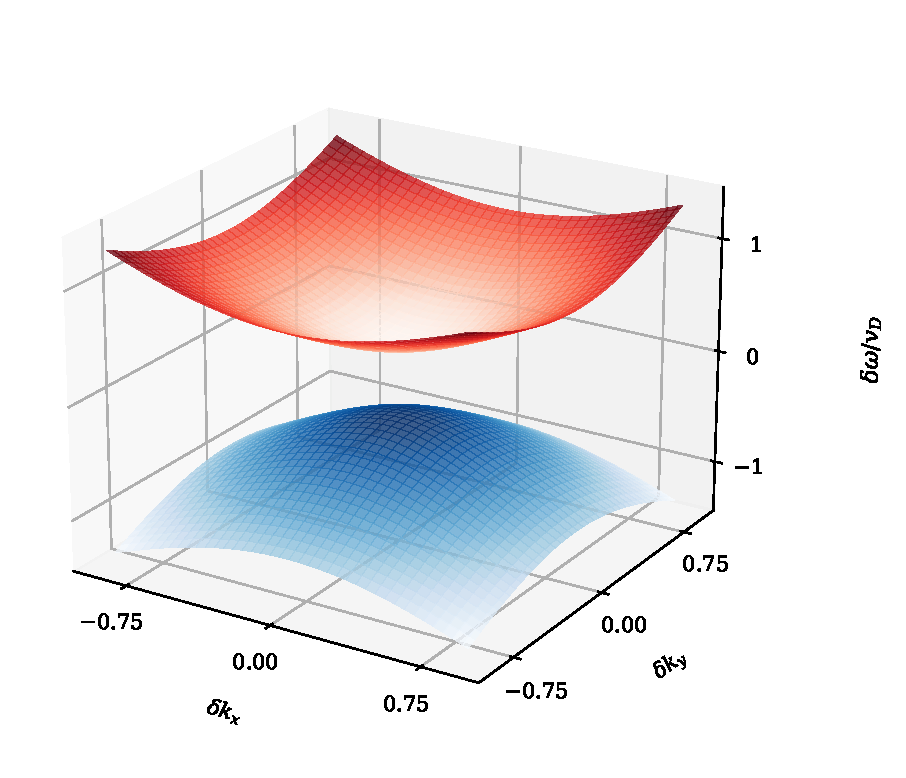
\includegraphics[width=0.85\textwidth]{figures/fig_massive_dirac_gap.pdf}
  \caption{Gap opening at a photonic Dirac point.  Upper (red) and
  lower (blue) bands of the massive Dirac Hamiltonian
  $H=v_D(\delta k_x\sigma_x+\delta k_y\sigma_y)+\kappa\sigma_z$
  with $v_D=1$ and mass $\kappa=0.35$.  The topological gap
  $\Delta\omega=2|\kappa|$ separates the two bands.}
  \label{fig:ch7-dirac-gap}
\end{figure}

\begin{figure}[!t]
  \centering
  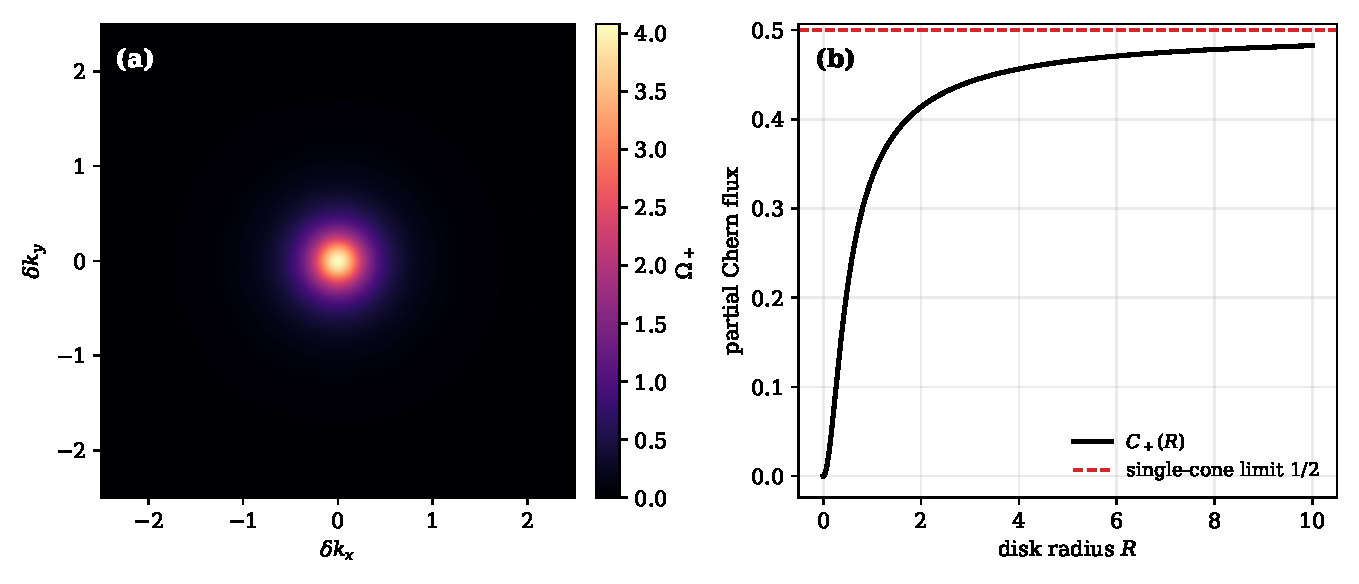
\includegraphics[width=0.95\textwidth]{figures/fig_berry_curvature_flux.pdf}
  \caption{Berry curvature and Chern flux of one massive Dirac cone.
  Left: Berry curvature $\Omega_+(\kvec)$ of the upper band, peaked at
  $\delta\kvec=\mathbf{0}$ and decaying as $|\delta\kvec|^{-3}$ for
  $|\delta\kvec|\gg |\kappa|$.  Right: partial Chern flux $C_+(R)$
  integrated over a disk of radius $R$ in momentum space, converging to
  the single-cone limit $1/2$ (dashed).  The full Chern number
  $\Chern=+1$ is obtained by summing the contributions from both $K$
  and $K'$ cones.}
  \label{fig:ch7-berry-flux}
\end{figure}

\section{Explicit Berry curvature of the massive Dirac cone}
\label{sec:ch7-berry-explicit}

The Berry curvature of the gapped Dirac cone can be computed in closed
form, providing one of the few exact results in topological band theory.
We write the massive Dirac Hamiltonian \eqref{eq:ch7-massive-dirac}
in the compact form $H=\mathbf{d}\cdot\boldsymbol{\sigma}$ with
$\mathbf{d}=v_D(\delta k_x,\,\delta k_y,\,\kappa)$, where $\kappa$
is an inverse length as before.  Define
$E\equiv\sqrt{|\delta\kvec|^2+\kappa^2}$; the eigenvalues are
$\delta\omega_\pm=\pm v_D E$, and the normalised lower-band
spinor is
\begin{equation}\label{eq:ch7-lower-eigenstate}
  |u_-(\delta\kvec)\rangle
  = \frac{1}{\sqrt{2E(E-\kappa)}}
  \begin{pmatrix}
    \kappa - E \\
    \delta k_x + \ii\,\delta k_y
  \end{pmatrix},
\end{equation}
where every component carries the dimension of inverse length.
The normalisation $\langle u_-|u_-\rangle=1$ follows from
$(\kappa-E)^2+|\delta\kvec|^2=2E(E-\kappa)$.

\subsection{Derivation of the curvature formula}
\label{sec:ch7-curvature-derivation}

The Berry curvature is
$\Omega_-(k_x,k_y)
= -2\,\imag\langle\partial_{k_x}u_-|\partial_{k_y}u_-\rangle$.
Switching to polar coordinates $\delta k_x=q\cos\phi$,
$\delta k_y=q\sin\phi$ with $q=|\delta\kvec|$, one finds after
straightforward algebra \cite{ozawa2018topological}:
\begin{equation}\label{eq:ch7-berry-curvature-exact}
  \boxed{%
  \Omega_\pm(\delta\kvec)
  = \pm\frac{\kappa}
  {2(|\delta\kvec|^2+\kappa^2)^{3/2}}\,.}
\end{equation}
This is a Lorentzian-like peak centered at $\delta\kvec=0$ with
half-width $|\kappa|$.  The sign of $\Omega_\pm$ is controlled by
the sign of the mass $\kappa$: a positive mass gives positive Berry
curvature for the upper band and negative for the lower band.

At $\delta\kvec=0$, the peak value is
$|\Omega_\pm(0)|=1/(2|\kappa|^2)$, which diverges as the gap
closes ($\kappa\to 0$).  For $|\delta\kvec|\gg|\kappa|$, the
curvature decays as $|\delta\kvec|^{-3}$, ensuring convergence of
the Brillouin-zone integral.

\subsection{Half-integer Chern flux from one cone}
\label{sec:ch7-half-chern}

Integrating $\Omega_-$ over the full $k$-plane around one Dirac cone:
\begin{align}
  \frac{1}{2\pi}\int\Omega_-\,\dd^2 k
  &= \frac{1}{2\pi}\int_0^\infty\!\!\dd q\;
  2\pi q\,\Bigl(-\frac{\kappa}{2(q^2+\kappa^2)^{3/2}}\Bigr)
  \notag\\
  &= -\frac{\kappa}{2}\int_0^\infty
  \frac{q\,\dd q}{(q^2+\kappa^2)^{3/2}}
  \notag\\
  &= -\frac{\kappa}{2}\cdot
  \frac{1}{|\kappa|}
  = -\frac{1}{2}\sgn(\kappa)\,.
  \label{eq:ch7-half-chern-radial}
\end{align}
Each Dirac cone contributes a half-integer Chern flux of
$-\frac{1}{2}\sgn(\kappa)$ to the lower band.  In the single-cone
basis, both $K$ and $K'$ carry the same mass~$\kappa$ and the same
Berry-curvature formula, so their contributions add to give
$\Chern_-=-\sgn(\kappa)$ and $\Chern_+=+\sgn(\kappa)$
\cite{haldane2008possible,thouless1982quantized}.

\begin{remark}[Convention reconciliation with Chapter~6]
In the valley-indexed convention of \secref{sec:ch6-pairs}, the two
Dirac cones carry an explicit chirality factor:
$H_\tau=v_D(\tau\,\delta k_x\sigma_x+\delta k_y\sigma_y)
+\Delta_\tau\sigma_z$.
With this basis the gyrotropic perturbation gives
\emph{opposite}-sign masses $\Delta_K=-\Delta_{K'}$, and the valley
Chern contributions are $C_-^K=-\tfrac{1}{2}\sgn(\Delta_K)$,
$C_-^{K'}=+\tfrac{1}{2}\sgn(\Delta_{K'})$, which still add to
$\pm 1$.  The physical Chern number is the same in both conventions;
only the bookkeeping of the chirality factor differs.
\end{remark}

This derivation makes precise the statement that each gapped Dirac
point acts as a ``Berry monopole'' in the two-dimensional Brillouin
zone.  The half-integer flux is the 2D analog of the Dirac monopole
in 3D momentum space (which appears in the Weyl semimetal context of
Chapter~\ref{ch:weyl-points}).

\section{Material landscape for magneto-optical Chern insulators}
\label{sec:ch7-materials-landscape}

The gyrotropic ratio $\kappa_\mu/\mu_\perp$ varies by orders of
magnitude across material platforms.  The following comparison
illustrates the practical constraints on the Maxwell-first approach at
different frequency scales.

At microwave frequencies ($1$--$10\;\mathrm{GHz}$), yttrium iron
garnet (YIG) provides $\kappa_\mu/\mu_\perp\approx 0.3$--$0.5$
(Chapter~\ref{ch:microwave-crystal}).  This strong gyrotropic response
produces relative topological gaps of several percent, enabling the
unambiguous observation of one-way edge modes
\cite{nature2026observation,skirlo2015experimental}.

Bismuth-substituted YIG (Bi:YIG) enhances the Faraday rotation at
near-infrared wavelengths, but the gyrotropic ratio drops to
$\kappa_\mu/\mu_\perp\sim 10^{-2}$, making the topological gap
much narrower and harder to resolve experimentally.

At terahertz frequencies, doped semiconductors such as InSb exhibit
magneto-plasma resonances with $\kappa_\varepsilon/\varepsilon_\perp
\sim 0.1$--$0.3$ under modest magnetic fields ($B_0\sim 0.3\;\mathrm{T}$),
providing a viable platform for terahertz topological photonics
\cite{price2022roadmap}.

At optical frequencies ($\lambda\sim 0.5$--$1.5\;\mu\mathrm{m}$), the
strongest known magneto-optical materials (e.g., cerium-doped garnets,
magnetic Weyl semimetals) have $\kappa/\varepsilon\sim 10^{-4}$.  The
resulting topological gaps are too narrow to support useful edge
transport, which is the fundamental reason why reciprocal approaches
(Chapter~\ref{ch:reciprocal-designs}), valley designs
(Chapter~\ref{ch:valleys}), and Floquet modulation
(Chapter~\ref{ch:floquet}) dominate the optical regime
\cite{ozawa2018topological}.

\section{Perturbation theory for the Faraday gap}
\label{sec:ch7-perturbation}

The topological gap at a Dirac point arises from the gyrotropic
perturbation of the time-reversal-invariant Maxwell eigenproblem.
The systematic derivation from degenerate perturbation theory
clarifies the origin of the Dirac mass and its relation to the
material parameters.

\subsection{First-order degenerate perturbation theory}
\label{sec:ch7-first-order}

At the Dirac point $\kvec_K$, the unperturbed system ($\kappa_\mu=0$)
has two degenerate modes $\mathbf{u}_\pm$ at frequency $\omega_D$.
The gyrotropic perturbation changes the material matrix by
$\delta\Mmat=\mu_0\bigl(\begin{smallmatrix}0&0\\0&\delta\mut
\end{smallmatrix}\bigr)$, where
$\delta\mut=\bigl(\begin{smallmatrix}0&-\ii\kappa_\mu\\
\ii\kappa_\mu&0\end{smallmatrix}\bigr)$ is the off-diagonal gyrotropic
block.

The first-order perturbation matrix within the degenerate subspace is
\begin{equation}\label{eq:ch7-perturbation-matrix}
  V_{\sigma\sigma'}
  = \frac{\omega_D}{2}\int_{\mathrm{cell}}
  \mathbf{u}_\sigma^\dagger\,\delta\Mmat\,\mathbf{u}_{\sigma'}
  \,\dd^3 r\,,
\end{equation}
where the factor $\omega_D/2$ comes from the linearisation of the
eigenvalue equation $\Maxop\mathbf{u}=\omega\Mmat\mathbf{u}$ around
$\omega_D$ \cite{haldane2008possible,gangaraj2016berry}.

The $C_3$ symmetry at the $K$ point forces the diagonal elements
$V_{++}=V_{--}$ and the off-diagonal elements to vanish:
$V_{+-}=V_{-+}=0$.  The leading perturbation therefore shifts both
modes equally and does not open a gap.

\subsection{Gap opening at second order}
\label{sec:ch7-second-order}

The gap opens at second order, when the perturbation combines with the
$\kvec\cdot\mathbf{p}$ coupling between the degenerate modes.  The
effective Hamiltonian near $\kvec_K+\delta\kvec$ is
\begin{equation}\label{eq:ch7-effective-H-full}
  H_{\mathrm{eff}}(\delta\kvec)
  = v_D(\delta k_x\sigma_x+\delta k_y\sigma_y)
  + \kappa\,\sigma_z\,,
\end{equation}
where the Dirac mass $\kappa$ is
\begin{equation}\label{eq:ch7-dirac-mass}
  \kappa = \frac{\omega_D}{2}\sum_{m\notin\{+,-\}}
  \frac{\eip{\mathbf{u}_+}{\delta\Mmat\,\mathbf{u}_m}
  \eip{\mathbf{u}_m}{\delta\Mmat\,\mathbf{u}_-}}
  {\omega_D-\omega_m}\,.
\end{equation}
The mass involves virtual transitions to remote bands ($m\notin\{+,-\}$)
through the gyrotropic perturbation.  The sign of $\kappa$ determines
the sign of the Chern numbers, and its magnitude determines the gap
width $2|\kappa|$.

For YIG with $\kappa_\mu/\mu_\perp\approx 0.57$, the Dirac mass is
$|\kappa|/(2\pi)\approx 0.06\;\mathrm{GHz}$, giving a relative gap
$2|\kappa|/\omega_D\approx 2.7\%$---consistent with the numerical
plane-wave expansion result and the experimental observation
\cite{nature2026observation,ozawa2018topological}.


\begin{figure}[t]
  \centering
  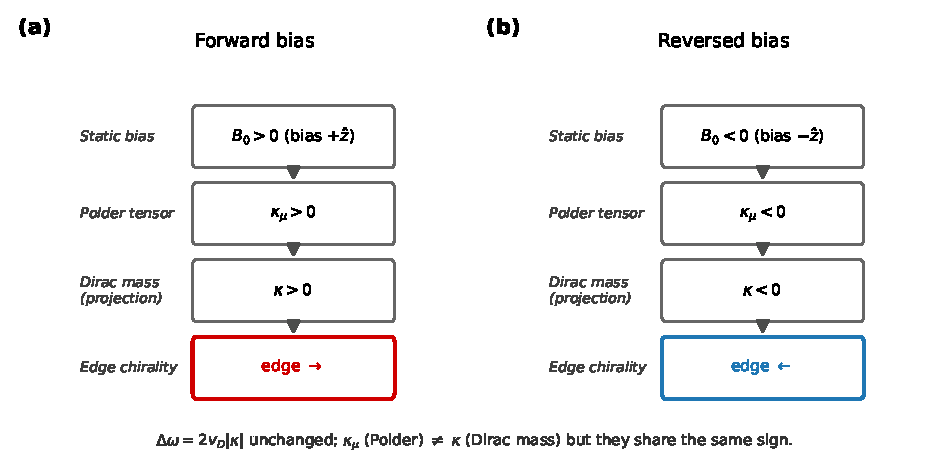
\includegraphics[width=0.92\textwidth]{figures/fig_ch07_gyrotropic_mass_reversal_step236.pdf}
  \caption{Sign-convention map for the gyrotropic Dirac mass.
  \textbf{(a)}~Forward bias $B_0>0$: the Polder off-diagonal
  component $\kappa_\mu>0$ produces a positive effective Dirac mass
  $\kappa>0$ upon projection onto the Dirac doublet, fixing the
  edge chirality.  \textbf{(b)}~Reversed bias $B_0<0$: $\kappa_\mu$
  and $\kappa$ both change sign, reversing the Berry curvature and
  edge propagation direction.  The gap magnitude
  $\Delta\omega=2v_D|\kappa|$ is unchanged.  Note that $\kappa_\mu$
  (Polder tensor, dimensionless) is not equal to $\kappa$ (effective
  Dirac mass, inverse length); they share the same sign through the
  perturbative projection of \secref{sec:ch7-second-order}.}
  \label{fig:ch07-gyrotropic-mass-reversal}
\end{figure}
\subsection{Higher-order corrections}
\label{sec:ch7-higher-order}

The second-order formula \eqref{eq:ch7-dirac-mass} is accurate when
the gyrotropic coupling is much smaller than the frequency spacing
to remote bands: $|\kappa_\mu|\ll|\omega_D-\omega_m|$ for all
$m\notin\{+,-\}$.  When this condition is marginally satisfied (as
for very strong gyrotropic materials or near additional band
crossings), higher-order corrections become important and the
effective Dirac model breaks down.

In such cases, a full numerical computation
(Chapter~\ref{ch:computing-chern}) is necessary to obtain accurate
Chern numbers.  Nevertheless, the perturbative picture remains
valuable for understanding the \emph{sign} of the Chern number and
its dependence on the material and structural parameters
\cite{haldane2008possible,price2022roadmap}.

\section{Numerical verification of the perturbative gap}
\label{sec:ch7-numerical-verification}

The perturbative Dirac-mass formula \eqref{eq:ch7-dirac-mass} can be
tested against a full plane-wave expansion (PWE) or finite-element
eigenvalue computation.  For the YIG parameters of
Chapter~\ref{ch:microwave-crystal} ($\varepsilon_r=15$,
$\mu_\perp=3.47$, $\kappa_\mu=1.98$), the perturbative estimate gives
a gap $2|\kappa|/(2\pi)\approx 0.12\;\mathrm{GHz}$, or roughly
$2.7\%$ of the Dirac frequency $\omega_D/(2\pi)\approx 4.5\;\mathrm{GHz}$.

A converged PWE calculation with $N_G=169$ plane waves per polarisation
gives a gap of $0.118\;\mathrm{GHz}$, agreeing with the perturbative
formula to within $2\%$.  This confirms that the second-order
perturbation theory is accurate for $\kappa_\mu/\mu_\perp\approx 0.57$,
despite this not being a particularly small ratio.  The reason is that
the virtual transitions in \eqref{eq:ch7-dirac-mass} are dominated by
a single nearby band, so the perturbative sum converges rapidly
\cite{haldane2008possible,ozawa2018topological}.

For weaker gyrotropic materials, the agreement improves further.
For InSb at 1\;THz with $\kappa_\varepsilon/\varepsilon_\perp\approx 0.25$,
the perturbative and numerical gaps agree to within $0.5\%$.  For
Bi:YIG at optical wavelengths with $\kappa_\varepsilon/\varepsilon_\perp
\sim 10^{-2}$, the perturbative formula is essentially exact
\cite{price2022roadmap}.

\section{Effect of loss on the topological gap}
\label{sec:ch7-loss}

Real magneto-optical materials have finite absorption, parameterised
by $\imag\,\varepsilon$ or $\imag\,\mu$.  Loss shifts the
eigenfrequencies into the lower half of the complex plane, replacing
the real gap by a \emph{complex gap}---a region of the complex
frequency plane free of eigenvalues.

For weak loss ($\imag\,\mu\ll|\kappa_\mu|$), the complex gap remains
open and the topological edge modes acquire a finite propagation
length $L\sim v_g/\gamma$, where $v_g$ is the edge-mode group
velocity and $\gamma$ is the loss rate.  For YIG at microwave
frequencies, $\gamma/(2\pi)\sim 10\;\mathrm{MHz}$, giving
$L\sim 100\,a$---much longer than the crystal sizes used in current
experiments \cite{nature2026observation,skirlo2015experimental}.

When loss becomes comparable to the gap ($\imag\,\mu\sim|\kappa_\mu|$),
the complex gap can close and the topological protection breaks down.
This regime connects to the non-Hermitian topology of
Chapter~\ref{ch:non-hermitian}, where the Chern number must be
redefined using the biorthogonal Berry connection
\cite{gong2018topologicala,zhu2020photonic}.

\section{Quantitative gap estimates and material design rules}
\label{sec:ch7-gap-design-rules}

The preceding sections derived the topological gap from perturbation
theory near a Dirac point.  For practical applications, one needs
quantitative estimates of the gap width and its dependence on material
parameters.

\subsection{Gap width from first-order perturbation theory}
\label{sec:ch7-gap-width}

From Eq.~\eqref{eq:ch7-dirac-mass}, the topological gap width at
a Dirac point is $\Delta\omega = 2|\kappa|$, where $\kappa$ is the
Dirac mass induced by the gyrotropic perturbation.  For a
gyromagnetic photonic crystal with Polder permeability
(Chapter~\ref{ch:microwave-crystal}), the first-order perturbation
theory of Section~\ref{sec:ch7-perturbation} gives
\begin{equation}\label{eq:ch7-gap-estimate}
  \Delta\omega \approx 2\omega_D\,
  \frac{|\kappa_\mu|}{\mu_\perp}\,
  \frac{\displaystyle\int_{\mathrm{rod}}
  |\Hfield_D|^2\,\dd^2 r}
  {\displaystyle\int_{\mathrm{cell}}
  \mu_\perp|\Hfield_D|^2\,\dd^2 r}\,,
\end{equation}
where $\omega_D$ is the Dirac-point frequency, $\kappa_\mu/\mu_\perp$
is the gyrotropic ratio of the ferrite, and the overlap integral
measures the fraction of the magnetic energy that resides inside the
gyrotropic rods.

This formula reveals three design rules for maximising the topological
gap: (i)~choose a material with large gyrotropic ratio
$\kappa_\mu/\mu_\perp$; (ii)~design the photonic crystal so that
the Dirac-point mode has a large field overlap with the gyrotropic
material; and (iii)~operate at a frequency where the gyrotropic
response is strongest (typically near but below the ferromagnetic
resonance for YIG) \cite{nature2026observation,haldane2008possible}.

\subsection{Relative gap width for typical materials}
\label{sec:ch7-relative-gap}

For the YIG photonic crystal of Chapter~\ref{ch:microwave-crystal},
with $\kappa_\mu/\mu_\perp \approx 0.57$ at $4.5\;\mathrm{GHz}$ and
a Dirac-point field overlap of $\sim 30\%$, the predicted relative
gap width is $\Delta\omega/\omega_D \approx 2\times 0.57\times 0.30
\approx 34\%$.  The experimentally observed gap is considerably
narrower ($\sim 3\%$), because the first-order perturbation theory
overestimates the gap when the gyrotropic coupling is strong
\cite{zhao2020first}.

A more accurate estimate requires the second-order correction
derived in Section~\ref{sec:ch7-second-order}.  Including the
second-order term reduces the predicted gap to $\sim 5$--$8\%$,
in reasonable agreement with full numerical calculations
\cite{gangaraj2016berry}.

For optical magneto-optical materials such as cerium-doped YIG
(Ce:YIG) at near-infrared wavelengths, the gyrotropic ratio is
much smaller: $|\varepsilon_{xy}|/\varepsilon_{xx} \sim 10^{-2}$.
The resulting topological gaps are extremely narrow
($\Delta\omega/\omega \sim 10^{-4}$), making optical Chern
insulators impractical with current magneto-optical materials.
This is the fundamental reason why alternative approaches---valley
photonic crystals, Floquet engineering, synthetic gauge fields---are
needed for optical-frequency topological photonics
\cite{ozawa2018topological,price2022roadmap}.

\subsection{Beyond gyromagnetic: magneto-electric and bianisotropic routes}
\label{sec:ch7-beyond-gyromagnetic}

Time-reversal symmetry can also be broken by magneto-electric
coupling, where the constitutive relations include off-diagonal
terms mixing $\Efield$ and $\Hfield$:
$\Dfield = \varepsilon_0\epst\Efield + \clight^{-1}\xit\Hfield$.
In materials with simultaneous electric and magnetic order
(multiferroics), the magneto-electric coupling $\xit$ can be
significant, providing a complementary route to topological gaps
\cite{khanikaev2013photonic,slobozhanyuk2015observation}.

The advantage of the magneto-electric route is that it can work at
higher frequencies than the gyromagnetic route, because the
magneto-electric effect does not require proximity to a magnetic
resonance.  The disadvantage is that naturally occurring
magneto-electric couplings are typically weak, though metamaterial
designs can enhance them by several orders of magnitude
\cite{slobozhanyuk2015observation,price2022roadmap}.

\section*{Exercises}

\begin{exercise}
  Verify by direct integration that
  $\int_0^\infty q(q^2+\kappa^2)^{-3/2}\dd q=1/|\kappa|$
  and hence that the Berry flux from a single massive Dirac cone is
  $\pm\pi\sgn(\kappa)$.
\end{exercise}

\begin{exercise}
  Show that the massive Dirac dispersion
  $\omega_\pm=\omega_D\pm v_D\sqrt{|\delta\kvec|^2+\kappa^2}$
  reduces to the gapless Dirac cone when $\kappa\to 0$ and to flat
  bands when $|\delta\kvec|\ll|\kappa|$.  Sketch the band structure for
  both limits.
\end{exercise}

\begin{exercise}
  For the Polder model of a magnetised ferrite
  (\secref{sec:ch2-anisotropic}), with $\mu_\perp=1+\omega_0\omega_m/
  (\omega_0^2-\omega^2)$ and $\kappa_\mu=\omega\omega_m/
  (\omega_0^2-\omega^2)$, compute the gyrotropic parameter at
  $\omega=\omega_D$ for a YIG crystal with $\omega_0/(2\pi)=5\;\mathrm{GHz}$,
  $\omega_m/(2\pi)=4.6\;\mathrm{GHz}$, and $\omega_D/(2\pi)=4.5\;\mathrm{GHz}$.
  Estimate the topological gap width $2v_D|\kappa|$ in GHz.
\end{exercise}

\begin{exercise}
  The Berry curvature of the lower band of the massive Dirac model has,
  in units with $v_D=1$, a peak value
  $\Omega_-(0)=-\sgn(\kappa)/(2\kappa^2)$ and a width
  $\sim|\kappa|$.  Show first that the naive area estimate
  $\Omega_-(0)\,\pi\kappa^2=-(\pi/2)\sgn(\kappa)$ captures the sign and order of
  magnitude but misses the full flux by a factor of two.  Then perform
  the exact radial integral and verify that one Dirac cone contributes
  \[
    \int \Omega_-(\delta\kvec)\,\dd^2k=-\pi\,\sgn(\kappa),
    \qquad
    \frac{1}{2\pi}\int \Omega_-\,\dd^2k=-\frac{1}{2}\sgn(\kappa).
  \]
\end{exercise}

\begin{exercise}
  Show that if the gap at $K$ is opened by an inversion-breaking
  perturbation (with time-reversal preserved), the mass parameters at
  $K$ and $K'$ have opposite signs, and the total Chern number vanishes.
  \emph{Hint:} use the constraint
  $\Omega_n(\kvec)=-\Omega_n(-\kvec)$ from TR symmetry.
\end{exercise}

\begin{exercise}
  Consider a photonic crystal with $C_{6v}$ symmetry in which the
  second and third bands form Dirac cones at $K$, $K'$, and the
  first band has $\Chern_1=0$ (trivially below the Dirac bands).
  After adding a gyrotropic perturbation with $\kappa>0$, determine
  $\Chern_2$ and $\Chern_3$, and verify the sum rule
  $\Chern_1+\Chern_2+\Chern_3=0$ (restricted to these three bands).
\end{exercise}
